\documentclass[a4paper,12pt]{report}
\usepackage{graphicx} % Required for inserting images
\usepackage[utf8]{vietnam} 
\usepackage{mathtools}
\usepackage{tabto}
\usepackage{graphicx}


\title{BÁO CÁO VI TÍCH PHÂN 2B}
\author{Đặng Duy Lân - 22120182\\Trần Thảo Ngân - 22120225}


\begin{document}
\maketitle
\section*{Bài 4.2.18}
a/ Vì nước được cho thoát ra với tốc độ 10 lít/phút
\\
$\Rightarrow$ Thể tích dung dịch thoát ra từ thời điểm \emph{t} đến thời điểm $\Delta$\emph{t} là 10$\Delta$\emph{t} lít (hay 10$\Delta$\emph{t} kg). 

Có $S(t)$ là lượng muối còn lại sau $t$ phút và $S(t + \Delta t)$ là lượng muối còn lại sau $t + \Delta t$ phút
\\
$\Rightarrow$ Lượng muối đã thoát ra là $S(t) - S(t + \Delta t)$ (kg).
\\
b/ Theo đề ta có bất đẳng thức:
\begin{align}
    \frac{S(t)}{100}(10\Delta t) \ge S(t) - S(t + \Delta t) \ge \frac{S(t + \Delta t)}{100}(10\Delta t)
\end{align}

Xét vế trái: $\frac{S(t)}{100}$ là \% muối còn lại trong nước sau $t$ phút
\\
$\Rightarrow$ $\frac{S(t)}{100} (10 \Delta t)$ là lượng muối có trong $10 \Delta t$ kg nước sau $t$ phút.

Xét vế phải: $\frac{S(t + \Delta t)}{100}$ là \% muối còn lại trong nước sau $t + \Delta t$ phút
\\
$\Rightarrow$ $\frac{S(t + \Delta t)}{100} (10 \Delta t)$ là lượng muối có trong $10 \Delta t$ kg nước sau $t + \Delta t$ phút.

Xét vế giữa: $S(t) - S(t + \Delta t)$ là lượng muối có trong $10\Delta t$ kg muối đã thoát ra.

Từ đó bất đẳng thức có nghĩa là: khi xét trên cùng 1 lượng nước (ở đây là $10\Delta t$ kg nước) thì lượng muối sau $t$ phút sẽ lớn hơn hoặc bằng lượng muối thoát ra trong $\Delta t$ phút và lớn hơn hoặc bằng lượng muối sau $t + \Delta t$ phút. Dấu "=" xảy ra khi $\Delta t = 0$.
\\
c/ Ta có: 
\begin{align*}
(1) \Longleftrightarrow \frac{S(t)}{100} \ge \frac{S(t) - S(t + \Delta t)}{10\Delta t} \ge \frac{S(t + \Delta t)}{100} \quad(\Delta t > 0)
\end{align*}

Khi $\Delta t \to 0$ thì $\frac{S(t + \Delta t)}{100} \to \frac{S(t)}{100}$, là 1 số dương hữu hạn. Do đó theo nguyên lý kẹp:
\begin{align*}
    &\lim_{\Delta t \to 0} \frac{S(t) - S(t + \Delta t)}{10\Delta t} = \frac{S(t)}{100}\\
    \Longleftrightarrow &\lim_{\Delta t \to 0} \frac{S(t) - S(t + \Delta t)}{\Delta t} = \frac{S(t)}{10}
\end{align*}

Đặt $y = S(t)$, khi đó
\begin{align*}
    \lim_{\Delta t \to 0} \frac{- \Delta y}{\Delta t} &= \frac{y}{10}\\
    \Longleftrightarrow -y' &= \frac{y}{10}
\end{align*}

Vậy phương trình vi phân lập được là: $-y' = \frac{y}{10}$ (2).
\\
d/ Viết lại (2) ta được:
\begin{align*}
    -\frac{dy}{dt} = \frac{y}{10}
\end{align*}

Do y là lượng muối có trong nước nên $y > 0$
\begin{align*}
    \Longrightarrow -\frac{dy}{y} = \frac{dt}{10}
\end{align*}

Tích phân 2 vế:
\begin{align*}
    \int\frac{-dy}{y} &= \int\frac{dt}{10}\\
    \Longleftrightarrow -ln(y) + C_1 &= \frac{t}{10} + C_2\\
    \Longleftrightarrow ln(y) &= \frac{-t}{10} + C\\
    \Longleftrightarrow y &= e^{\frac{-t}{10} + C}
\end{align*}

Lại có $y(0) = 10$ $\Longrightarrow 10 = e^{C} \Longrightarrow C = ln(10)$ 

Vậy $S(t) = e^{\frac{-t}{10} + ln(10)} = 10 \cdot e^{\frac{-t}{10}}$
\\
e/ Sau 30 phút, lượng muối còn lại trong hồ là: $S(30) = 10 \cdot e^{\frac{-30}{10}} \approx 0.5$(kg)

\section*{Bài 2}
Ta có:
\begin{align*}
    &y' + \frac{1}{3}y = e^{x}y^{4}\\
    \Longleftrightarrow &\frac{y'}{y^{4}} + \frac{1}{3y^{3}} = e^{x}\\
    \Longleftrightarrow &\frac{y^{-4}dy}{dx} + \frac{1}{3y^{3}} = e^{x}
\end{align*}
Đặt $u = y^{-3} \Longrightarrow du = -3y^{-4}dy$:
\begin{align*}
    (*) &\Longleftrightarrow \frac{du}{-3dx} + \frac{u}{3} = e^{x}\\
    &\Longleftrightarrow u' - u = -3e^{x}
\end{align*}
Nhân cả 2 vế cho $e^{-x}$ ta được:
\begin{align*}
    &u'e^{-x} - u.e^{-x} = -3\\
    \Longleftrightarrow &(u.e^{-x})' = -3\\
    \Longleftrightarrow &\frac{d}{dx}(u.e^{-x}) = -3\\
    \Longleftrightarrow &d(u.e^{-x}) = -3dx
\end{align*}
Tích phân 2 vế:
\begin{align*}
    &\int d(u.e^{-x}) = \int -3dx\\
    \Longleftrightarrow &u.e^{-x} = -3x + C\\
    \Longleftrightarrow &u = e^{x}(-3x + C)\\
    \Longleftrightarrow &y^{-3} = e^{x}(-3x+C)\\
    \Longleftrightarrow &y = \frac{1}{(e^{x}(-3x + C))^{\frac{1}{3}}}
\end{align*}
Lại có $y(0) = 1 \Rightarrow \frac{1}{C} = 1 \Leftrightarrow C = 1$.
\\
Vậy $y = \frac{1}{(e^{x}(-3x + 1))^{\frac{1}{3}}}$
\\ \\
\textbf{Dùng phần mềm Matlab để thử lại:}

Câu lệnh: dsolve$('Dy + y/3 = exp(x) * y \hat{\hspace{7pt}} 4', \hspace{5pt} 'y(0) = 1', \hspace{5pt} 'x')$

Kết quả:
\begin{figure}[h]
    \centering
    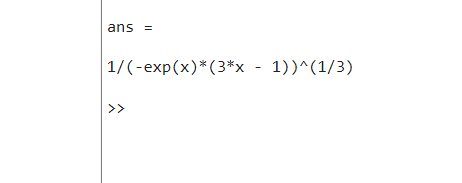
\includegraphics{answer.png}
\end{figure}
\\
\textbf{Vẽ đồ thị bằng phần mềm Geogebra:}
\newpage
Nhập hàm số:
\begin{figure}[h]
    \centering
    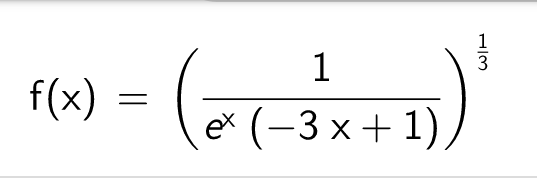
\includegraphics [scale = 0.7] {graph_input.png}
\end{figure}

Đồ thị được vẽ ra:
\begin{figure}[ht]
    \centering
    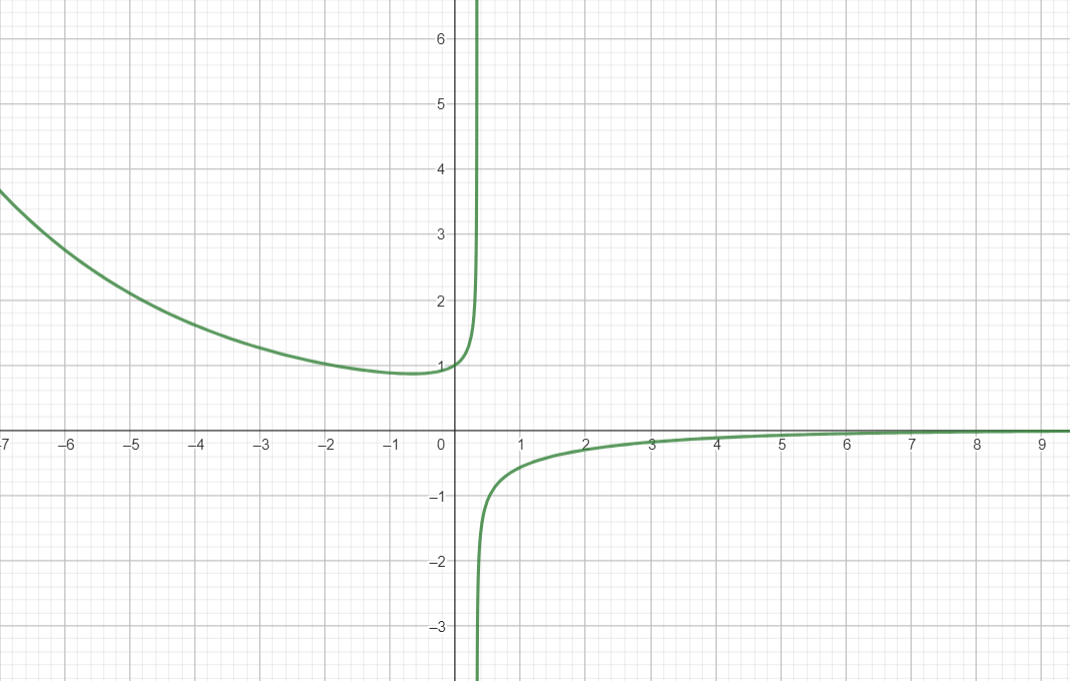
\includegraphics [scale = 0.6] {graph.png} 
\end{figure}

\end{document}
